%% Template para dissertacao/tese na classe UFBAthesis
%% versao 1.0
%% (c) 2005 Paulo G. S. Fonseca
%% (c) 2012 Antonio Terceiro
%% (c) 2014 Christina von Flach
%% www.dcc.ufba.br/~flach/ufbathesis

%% Carrega a classe ufbathesis
%% Opcoes: * Idiomas
%%           pt   - portugues (padrao)
%%           en   - ingles
%%         * Tipo do Texto
%%           bsc  - para monografias de graduacao
%%           msc  - para dissertacoes de mestrado (padrao)
%%           qual - exame de qualificacao de mestrado
%%           prop - exame de qualificacao de doutorado
%%           phd  - para teses de doutorado
%%         * Media
%%           scr  - para versao eletronica (PDF) / consulte o guia do usuario
%%         * Estilo
%%           classic - estilo original a la TAOCP (deprecated) - apesar de deprecated, manter esse.
%%           std     - novo estilo a la CUP (padrao)
%%         * Paginacao
%%           oneside - para impressao em face unica
%%           twoside - para impressao em frente e verso (padrao)

% Aten��o: Manter 'classic' na declaracao abaixo:
\documentclass[qual, classic, a4paper]{ufbathesis}

%% Preambulo:
\usepackage[utf8]{inputenc}
\usepackage{graphicx}
\usepackage{lipsum}
\usepackage{hyphenat}
\usepackage[usenames, dvipsnames, table]{xcolor}
\usepackage{booktabs}
\usepackage{pifont}
\usepackage{multirow}
\usepackage{listings} 
\usepackage{colortbl}
\usepackage{xfrac}
\usepackage[FIGTOPCAP]{subfigure}
\usepackage[printonlyused, withpage]{acronym}

% Universidade
\university{Universidade Federal da Bahia}

% Endereco (cidade)
\address{Salvador}

% Instituto ou Centro Academico
\institute{Instituto de Matem\'{a}tica}

% Nome da biblioteca - usado na ficha catalografica
\library{Biblioteca Reitor Mac\^{e}do Costa}

% Programa de pos-graduacao
\program{Programa de P\'{o}s-Gradua\c{c}\~{a}o em Ci\^{e}ncia da Computa\c{c}\~{a}o}

% Area de titulacao
\majorfield{Ci\^{e}ncia da Computa\c{c}\~{a}o}

% Titulo da dissertacao
\title{Detecção de mudanças de conceito em fluxos de dados não estacionários}

% Data da defesa
% e.g. \date{19 de fevereiro de 2013}
\date{19 de Julho de 2018}
% e.g. \defenseyear{2013}
\defenseyear{2018}

% Autor
% e.g. \author{Jose da Silva}
\author{***}

% Orientador(a)
% Opcao: [f] - para orientador do sexo feminino
% e.g. \adviser[f]{Profa. Dra. Maria Santos}
%\adviser{Ricardo Araújo Rios}
\adviser{***}

% Orientador(a)
% Opcao: [f] - para orientador do sexo feminino
% e.g. \coadviser{Prof. Dr. Pedro Pedreira}
% Comente se nao ha co-orientador
%\coadviser{Nome Completo do CO-ORIENTADOR}

%% Inicio do documento
\begin{document}

\pgcompfrontpage

%% Parte pre-textual
\frontmatter

\pgcomppresentationpage


%%%%%%%%%%%%%%%%%%%%%
% Resumo em Portugues
%%%%%%%%%%%%%%%%%%%%%

\resumo
O aprendizado a partir de fluxos de dados (aprendizagem incremental) tem crescido como foco de pesquisa, graças a existência de problemas práticos e desafios em aberto.
Dentre estes, está a detecção de mudanças de conceito, fenômeno que ocorre quando a distribução dos dados é alterada, tornando o modelo vigente impreciso ou obsoleto.
Neste trabalho, propomos uma nova técnica para detecção de mudanças de conceito.

% Palavras-chave do resumo em Portugues
\begin{keywords}
Mudança de conceito, detecção de mudanças, detecção de novidades, aprendizagem adaptativa, fluxos de dados.
\end{keywords}

%%%%%%%%%%%%%%%%%%%
% Resumo em Ingles
%%%%%%%%%%%%%%%%%%%

\abstract
Learning from data streams (incremental learning) is increasing as a research focus, due to the existence of practical problems and open challenges. Among which, is the detection of concept drift, a phenomenon that happens when the data distribution is altered, making the model inaccurate or obsolete. In this work, we propose a novel technic to detect concept drifts.

% Palavras-chave do resumo em Ingles
\begin{keywords}
Concept drift, change detection, adaptive learning, data streams.
\end{keywords}

%%%%%%%%%%%%%%%%%%%
% Sumario / Indice
%%%%%%%%%%%%%%%%%%%

% Comente para ocultar
\tableofcontents

% Lista de figuras
% Comente para ocultar
%\listoffigures

% Lista de tabelas
% Comente para ocultar
%\listoftables

%\chapter*{Lista de Siglas}

% Sintaxe da lista de acordo com a documentação do pacote `acronym'
% documentação: http://mirror.unl.edu/ctan/macros/latex/contrib/acronym/acronym.pdf
%\begin{acronym}[PGCOMP]
%    \acro{PGCOMP}{Programa de Pós-Graduação em Ciência da Computação}
    %\acro{CNPq}{Conselho Nacional de Desenvolvimento Científico e Tecnológico}
%\end{acronym}

%% Parte textual
\mainmatter

% Eh aconselhavel criar cada capitulo em um arquivo separado, digamos
% "capitulo1.tex", "capitulo2.tex", ... "capituloN.tex" e depois
% inclui-los com:
% \include{capitulo1}
% \include{capitulo2}
% ...
% \include{capituloN}
%
% Importante: 
% Use \xchapter{}{} ao inves de \chapter{}; se n�o quiser colocar texto antes do inicio do capitulo, use \xchapter{texto}{}.

% \xchapter{Introdu\c{c}\~{a}o}{Este eh o primeiro cap\'{\i}tulo, onde eu conto toda a historia deste trabalho, o problema, a solu\c{c}\~{a}o, etc.}

% É recomendável utilizar `\acresetall' no início de cada capítulo para reiníciar o contator de referências às siglas.
% \acresetall 


%\section{Se\c{c}\~{a}o}
%Trabalho do  \ac{PGCOMP}. Bolsa do \ac{CNPq}.

%\begin{figure}[h]
%Figure
%\caption{As siglas também funcionam nas legendas, seja na forma de sigla \ac{CNPq}, seja na forma completa \acf{PGCOMP}.}
%\end{figure}

%\lipsum

%\subsection{Uma Subse\c{c}\~{a}o}
%\acresetall
%Texto para mostrar como o \verb|\acresetall| funciona \ac{CNPq}, \ac{PGCOMP}. Ele reseta os contadoes e faz a sigla %aparecer na forma estendida novamente.

%\subsection{Outra Subse\c{c}\~{a}o}

%Texto  \acf{CNPq}, \acf{PGCOMP}.

\xchapter{Revis\~{a}o Bibliogr\'{a}fica}{}

\subsection{Introdução}

A extração de informações úteis a partir de grandes conjuntos de dados é uma tarefa desafiadora para os pesquisadores.
Os algoritmos de aprendizagem de máquina baseados em fluxos de dados contínuos (FCDs) atuam em um contexto diferente dos algoritmos tradicionais, 
devido à natureza dinâmica dos FCDs.
Esses algoritmos devem se adaptar às constantes mudanças na distribuição dos dados, para não se tornarem imprecisos ou obsoletos.

Logo, a atividade de Detecção de Novidades (DN) - \textit{Concept Drift Detection} - é essencial para o bom funcionamento dessas técnicas. Pois permite identificar o surgimento de novos conceitos e mudanças em conceitos existentes, viabilizando a atualização do modelo de decisão. Tamanha importânica tem motivado a exploração de novas técnicas de aprendizado ativo, com o objetivo de aprimorar o processo de classificação e identificação de mudanças de conceito. 

Este capítulo descreve as diferentes situações que estão presentes em FCDs e os principais algoritmos para detecção de novidades.

\subsection{Fluxos Contínuos de Dados}

Fluxos Contínuos de Dados (FCDs) podem ser definidos como sequências contínuas de dados, de tamanho ilimitado, sem ordem definida e de alta frequência \cite{Babcock:2002:MID:543613.543615}. O desenvolvimento de algoritmos de aprendizado para esses cenários é uma tarefa custosa, pois estes devem lidar com sequências de dados geradas de forma contínua, em alta velocidade e cuja distribuição pode sofrer alterações ao longo do tempo \cite{Gama:2014:survey}. 

Os avanços recentes em hardware e software permitiram a aquisição de dados em maior escala. Assim, a grande frequência e quantidade de dados coletados passaram a caracterizar os ambientes dinâmicos.  Ambientes estes que diferem completamente das bases de dados tradicionais, que supõem cenários estáticos. Os avanços tecnológicos também permitiram o surgimento de diversas aplicações do mundo real com essas características: 

\begin{itemize}
    \item \textbf{Sistemas de Segurança}: monitoramento contínuo através de imagens ou outros sensores para identificação de intrusos;

    \item \textbf{Redes de Computadores}: análise do tráfego de rede, monitorando pacotes distoantes, além de realizar a detecção de invasores;

    \item \textbf{Mercado Financeiro}: análise de dados e estatísticas, produzindo informações para investidores. Outra vertente importante é a detecção de fraudes;

    \item \textbf{Medicina}: aprimoramento do modelo de detecção de determinada doença a partir das análises e resultados de novos casos.
\end{itemize}

Conforme \cite{Gama:2014:survey}, as principais características dos fluxos contínuos de dados são:

\begin{itemize}
    \item \textbf{Contínuos}: elementos que compõem os dados são recebidos de forma continuada;

    \item \textbf{Não estacionário}: distribuição de probabilidade sofre alterações ao longo do tempo;

    \item \textbf{Potencialmente Infinitos}: os fluxos são potencionalmente infinitos, o que impede o completo armazenamento em memória.
\end{itemize}

Essas propriedades, sobretudo o fato de não serem estacionários, inviabilizam a aplicação dos algoritmos tradicionais de mineração de dados e aprendizagem de máquina em cenários com FCDs.

Por não serem estáticos, é comum que ocorram mudanças de conceito (\textit{concept drift}), que são mudanças na distribuição dos dados durante a execução da aplicação. A figura \ref{fig1} representa um caso clássico de mudança de conceito: a alteração do perfil de compra de um cliente.
A evolução de conceito (\textit{concept evolution}) caracteriza-se pelo surgimento de novas classes, diferentes das classes conhecidas. Cada nova classe representa uma evolução, por exemplo, um novo interesse do cliente. Todavia, para que seja possível aprimorar modelos baseados em FCDs, também é necessário esquecer conceitos desatualizados ou obsoletos, que apenas ocupam espaço e degradam o resultado das predições \cite{Abdallah}.

\begin{figure}[ht!]
    \begin{center}
      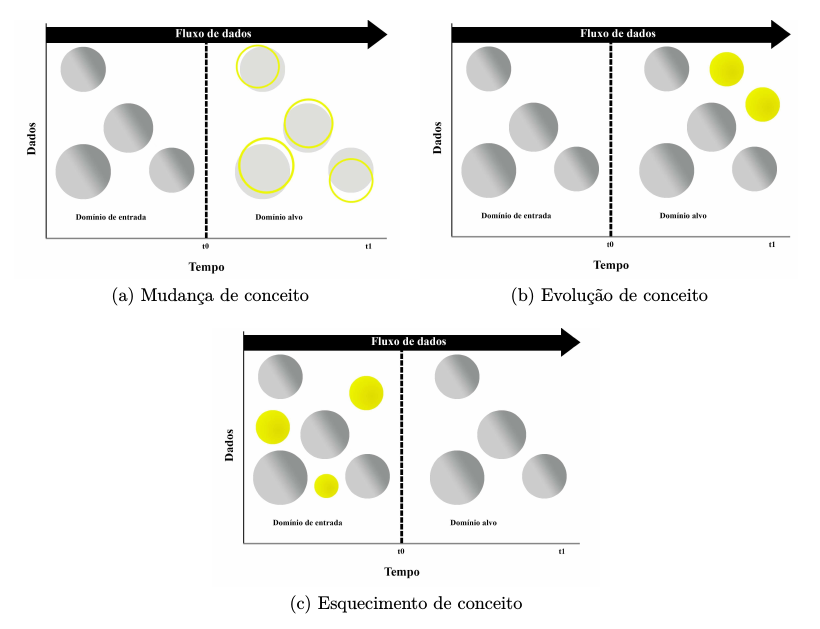
\includegraphics[scale=0.6]{001.png}
    \caption{Mudança de conceito - Exemplo: Perfil de Compra}
    \label{fig1}
    \end{center}
\end{figure}

\subsection{Algoritmos de classificação e FCDs}

Algoritmos de classificação aplicados a FCDs permitem predizer, com alta acurácia, a classe de novos exemplos obtidos a partir do fluxo de dados. 
Durante o aprendizado supervisionado, um conjunto de dados previamente rotulado é fornecido ao algoritmo, para construção do modelo. É a construção deste modelo que possibilita inferir a classe de novos exemplos que venham a ser encontrados. Contudo, é importante que o modelo seja constantemente atualizado (evolua), para que contemple e classifique de forma correta novas distribuições de dados.

Dentre os principais algoritmos de classificação para cenários tradicionais (informação em lote, \textit{batch}), estão: árvores de decisão, SVM e Naive Bayes. Estes algoritmos são aplicados em ambientes estacionários, isto é, em ambientes em que o modelo de decisão não requer atualizações frequentes e o algoritmo pode considerar que todos dados necessários podem ser armazenados em memória.

Entretanto, o aprendizado de novos conceitos a partir de fluxos contínuos de dados ocorre de forma significativamente diferente do modelo tradicional, estático. Para lidar com esse novo cenário, diversos algoritmos clássicos têm sido adaptados e novos algoritmos estão sendo desenvolvidos.

Algoritmos de aprendizagem de máquina com foco em FCDs geralmente atuam em duas fases: \textit{offline} e \textit{online}. Na fase \textit{offline}, o algoritmo recebe exemplos rotulados, que são utilizados na elaboração de um modelo de decisão ou atualização do modelo existente. Na fase \textit{online}, novos exemplos são classificados conforme são recebidos. Ao longo do tempo, o modelo construído é continuamente atualizado, para evitar a diminuição da acurácia ou a obsolência do modelo.

A maior dificuldade para os algoritmos de classificação em cenários FCDs é a detecção e o tratamento de mudanças de conceito \cite{Aggarwal:2006:DSM:1196418}, ou seja, mudanças na distribuição dos dados ao longo do tempo. 
Além desse, outros desafios precisam ser vencidos, tais como: incorporação de novos conceitos, detecção e remoção de \textit{outliers} e ruídos, além da manutenção de uma boa precisão paralelamente à evolução dos dados. Portanto, os algoritmos devem ter a capacidade de atualizar o modelo de decisão periodicamente, permitindo que a aplicação tenha um processo de aprendizagem contínuo.

O processo de atualização do modelo de decisão é um componente importante dos algoritmos de classificação em FCDs. Este melhoramento pode ser feito com ou sem \textit{feedback} externo. Algoritmos que utilizam \textit{feedback} externo assumem que o rótulo verdadeiro de todos exemplos estará disponível, mesmo que com um certo atraso. 
Nesta abordagem, o algoritmo atualiza o modelo de tempos em tempos, conforme novos rótulos de exemplos são obtidos. Os algoritmos que não utilizam \textit{feedback} em seu ciclo de atualização, não requerem a correta rotulação pós-processamento. Na abordagem sem \textit{feedback}, outros indicadores e métodos são utilizados para renovação do modelo. Uma terceira abordagem é a utilização parcial de \textit{feedbacks}. Neste caso, um conjunto parcial de rótulos é utilizado para atualizar o modelo.

\subsection{Detecção de Novidades em FCDs}

Detecção de novidade (\textit{concept drift detection}) consiste em identificar quando a distribuição dos dados de teste diverge da distribuição utilizada em treinamento. Esta é uma tarefa importante em classificação de FCDs, graças à natureza não-estacionária destes. A detecção de novidades tem como principal objetivo perceber novos padrões emergentes no fluxo de dados, possibilitando a identificação de novos conceitos, mudanças nos conceitos conhecidos e a presença de ruídos.

Na literatura recente, é possível encontrar algoritmos para classificação em cenários FCD com suporte à detecção de novidades (DN), dentre os mais referenciados estão: AnyNovel \cite{Abdallah}, ECSMiner \cite{Masud:2010:ACC:1933307.1934606}, CLAM \cite{malkhateeb} e OLINDDA \cite{Spinosa:2009:NDA:1551768.1551770}. O desenvolvimento de algoritmos para DN em cenários FCD tem como principais desafios:

\begin{itemize}
    \item \textbf{Mudança de Conceito}: dificulta a correta classificação dos exemplos ao longo do tempo;

    \item \textbf{Evolução de Conceitos}: novas classes surgem com o decorrer do tempo;

    \item \textbf{Contextos Recorrentes}: conceitos ora esquecidos ressurgem, podendo ser confudidos com novos conceitos;

    \item \textbf{Ruídos ou \textit{Outliers}}: pontos distoantes na distribuição que podem ser confudidos com novos conceitos.
\end{itemize}

Geralmente, a detecção de novidades (DN) ocorre durante a fase \textit{online}, através da detecção de exemplos que não podem ser identificados pelo modelo atual. Entretanto, algumas propostas simplesmente consideram estes exemplos como atípicos. Outras propostas, mais refinadas, salvam estes exemplos em uma memória temporária e utilizam-nos em uma análise futura, objetivando identificar o surgimento de uma novidade.

Apesar da maioria dos algoritmos para detecção de novidades em FCDs considerar que apenas uma classe nova pode surgir a cada janela de tempo considerada, alguns trabalhos como o ECSMiner \cite{Masud:2010:ACC:1933307.1934606}, entendem que diferentes padrões novos podem surgir a cada intervalo, sendo importante diferenciá-los.

Conforme já explicitado, a atualização do modelo pode utilizar ou não \textit{feedback} externo. Uma abordagem elegante, é a utilização de técnicas de aprendizado ativo para escolher, dentre os exemplos não classificados pelo modelo, quais devem ser rotulados e utilizados no processo de atualização. 

\subsection{Aprendizado Ativo e FCDs}

A tarefa de classificação pode utilizar uma metodologia chamada de aprendizagem ativa (\textit{active learning}), que possibilita ao algoritmo separar parte das instâncias e solicitar a correta rotulação a um especialista \cite{Tong:2001}. As instâncias rotuladas são então aplicadas no processo de atualização do modelo de decisão.  A utilização da técnica de aprendizagem ativa busca minimizar o custo de rotulação dos dados para atualização do modelo. É um estratégia interessante, sobretudo em cenários FCDs, pois não requer a rotulação de todos os dados para manutenção do modelo.

Por não contemplar todos os dados, o maior desafio da aprendizagem ativa reside em como selecionar as instâncias a serem rotuladas, para que se possa obter maior e melhor capacidade de previsão \cite{Tong:2001}.

Na literatura é possível obter uma lista das capacidades que as estratégias de aprendizagem ativa devem apresentar \cite{Ienco:2014}: 

\begin{itemize}
    \item Preservar a distribuição dos dados de entrada;
    \item Detectar onde ocorrem as mudanças ao longo do fluxo de dados;
    \item Equilibrar, ao longo do tempo, o custo de realizar a rotulação das instâncias.
\end{itemize}

Novos algoritmos têm sido desenvolvidos para lidar com a escassez de rótulos para atualização de modelos que lidam com fluxos contínuos. 
O particionamento dos fluxos em lotes é a principal estratégia adotada por essas novas abordagens. Assim, o processo de aprendizagem ativa se dá por lote, assumindo que os dados presentes em cada lote são estacionários. O objetivo é treinar um classificador mais preciso a partir de uma pequena porção dos dados, diminuindo o custo de rotulação.

Outra abordagem, também muito aplicada, é o agrupamento dos exemplos não classificados pelo modelo, considerando-os como potenciais novidades. Um representante de cada agrupamento é então rotulado e utilizado na atualização do modelo. Esta estratégia é aplicada no algoritmo AnyNovel \cite{Abdallah}.

\subsection{Algoritmos para DN em FCDs}

Os algoritmos para detecção de novidades em fluxos de dados contínuos são divididos em duas fases: \textit{offline} e \textit{online}. Na fase \textit{offline}, o modelo de decisão é construído a partir de dados previamente rotulados. Enquanto que na fase \textit{online}, este modelo é aplicado para inferir os exemplos recebidos a partir do fluxo. 

Nesta seção serão descritos alguns dos algoritmos para DN em FCDs presentes na literatura. Serão abordados os seguintes algoritmos: AnyNovel \cite{Abdallah}, ECSMiner \cite{Masud:2010:ACC:1933307.1934606}, CLAM \cite{malkhateeb} e OLINDDA \cite{Spinosa:2009:NDA:1551768.1551770}.

O AnyNovel \cite{Abdallah}, é um algoritmo para tratamento de \textit{concept drift}, especializado em um cenário específico: a identificação de atividades em fluxos de dados gerados por sensores. O algoritmo faz uso da metodologia de aprendizagem ativa. Os dados recebidos são armazenados em uma memória temporária. Esta memória é dividida em blocos que são liberados para análise apenas quando o número máximo de instâncias é atingido. O algoritmo, então, classifica os dados do bloco entre: existente, novidade ou desconhecido. A aprendizagem ativa, através de um especialista, ocorre quando blocos de novidade ou desconhecidos são encontrados.

O ECSMiner \cite{Masud:2010:ACC:1933307.1934606} realiza o tratamento de DNs em tarefas de classificação multiclasse. O ECSMiner constrói um comitê de classificadores de árvoes de decisão a partir de \textit{chunks} dos dados. Os nós-folhas das árvores construídas são agrupados.
Estes microgrupos são utilizados para explicar os exemplos do fluxo. Exemplos que não estejam enquadrados em nenhum subgrupo, são marcados como \textit{outliers} e armazenados para futura análise. 
Quando um número suficiente de \textit{outliers} é detectado, e estes \textit{outliers} formam um grupo distinto dos grupos já conhecidos, ocorre a identificação de uma novidade. A principal limitação do algoritmo é a suposição de que no máximo apenas uma novidade ocorrerá por \textit{chunk} de dados.

O algoritmo CLAM \cite{malkhateeb} atua de forma similar ao ECSMiner, mas ao invés de utilizar apenas um comitê, cria-se um comitê de classificadores para cada classe conhecida do problema.
Estes classificadores, por sua vez, são formados por microgrupos. A classificação de uma instância é realizada através da identificação de qual microgrupo apresenta o centro mais próximo desta. A cada exemplo, cada um dos comitês é testado como classificador. Se o comitê não conseguir classificar o exemplo, este é marcado como desconhecido. Contudo, um exemplo só é categorizado como desconhecido se a maioria dos comitês assim o considerar. Nesse caso,um novo conceito é detectado. Assim como o ECSMiner, o algoritmo pressupõe que somente um novo padrão será identificado por bloco de dados.

O OLLINDDA \cite{Spinosa:2009:NDA:1551768.1551770} utiliza um algoritmo de agrupamento para produzir \textbf{k} grupos, representados por centro e raio. Este conjunto de \textbf{k} grupos representa o modelo normal. 
Um macro-esfera também é criada para manter um macrogrupo dos grupos criados. Esta macro-esfera realiza a separação do modelo normal dos sub-modelos de extensão e novidade. 
Quando novos exemplos são classificados dentro da macro-esfera, eles são considerados como extensão. Se forem classificados fora da macro-esfera, são percebidos como novidade. 
A classificação de novos exemplos se dá pelo cálculo da distância do centroide do grupo encontrado até o centroide do grupo mais próximo.
Se a distância calculada for menor que o raio do grupo, este exemplo pode ser explicado pelo modelo atual, senão será marcado como desconhecido.

\subsection{Considerações Finais}

Neste capítulo foram apresentados alguns algoritmos para detecção de novidades em fluxos de dados contínuos. Verificou-se que a maior parte dos algoritmos lida com mudanças de conceito através da atualização periódica do modelo através de estratégias supervisionadas ou não supervisionadas.

Contudo, novos algoritmos utilizando a metodologia de aprendizagem ativa têm surgido. Nos trabalhos que apresentam tais metodologias, percebe-se a obtenção de maior eficácia, em relação à quantidade de erros na classificação e à capacidade preditiva do algoritmo.

%hline
%\end{tabular}
%\end{center}
%\label{default-table2}
%\end{table}%

%\xchapter{Outro cap\'{\i}tulo}{} %sem preambulo
%\lipsum


%% Parte pos-textual
\backmatter

% Bibliografia
% � aconselh�vel utilizar o BibTeX a partir de um arquivo, digamos "biblio.bib".
% Para ajuda na cria��o do arquivo .bib e utiliza��o do BibTeX, recorra ao
% BibTeXpress em www.cin.ufpe.br/~paguso/bibtexpress
\bibliographystyle{abntex2-alf}
\bibliography{biblio}

% Apendices
% Comente se naoo houver apendices
%\appendix

%\xchapter{Exemplo de Ap\^endice}{} %sem preambulo
%\lipsum
% Eh aconselhavel criar cada apendice em um arquivo separado, digamos
% "apendice1.tex", "apendice.tex", ... "apendiceM.tex" e depois
% inclui--los com:
% \include{apendice1}
% \include{apendice2}
% ...
% \include{apendiceM}

%% Fim do documento
\end{document}
%------------------------------------------------------------------------------------------%
